\part{Etudes des séjours dans une classe}
\section{Période de classe}
\subsection{Définition}
Soit C une classe d'équivalence pour $i\leftrightarrow j$.\\
\[C=cl\{i\}=cl\{j\},\ \forall i,j\in C\]

$\forall i,j\in C$, il existe un chemin (orienté) allant de $i$ à $j$. On appelera :
\begin{eqnarray*}
	N_{ij}&=&\{n>0;\text{ il existe un chemin allant de } i \text{ à } j \text{ de longueur } n\} \\
		&=&\{n>0;\ p^i_j(n)>0\}
\end{eqnarray*}

\Prop{fondamentale}{$i,j,k\in C$\\
Si $a\in N_{ij}$ et $b\in N_{jk}$ alors $a+b\in N_{ik}$, ie $N_{ij}+N_{jk}\subset N_{ik}$.}

\Theo{}{Soit $d_i=PGCD(N_{ii})$ pour $i\in C$.
\[\forall i,j\in C, d_i=d_j\]}

\begin{dem}
	Soient $a\in N_{jj}$, $b\in N_{ji}$ et $c\in N_{ij}$.
	\[a+b+c=c+a+b\in N_{ii}\]
	Or, $b+c=c+b\in N_{ii}$, donc :
	\[a+b+c\equiv0[d_i] \text{ et } b+c\equiv0[d_i] \Rightarrow a\equiv0[d_i]\ \forall a\in N_{jj}\]
	donc $d_j\equiv 0 [d_i]$ et de même, $d_i\equiv 0[d_j]$, donc $d_i=d_j$.
\end{dem}

\Def{Période d'une classe}{Notons $d$ cet entier commun à tous les $i\in C$. $d$ est appelé la \textit{période de la classe $C$}.\\
Si $d=1$, la classe est dite \textit{apériodique}.}

\newpage
\Exemp{}{\begin{minipage}{0.4\linewidth}
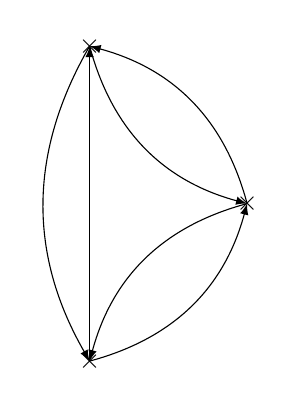
\begin{tikzpicture}
	\draw (0,4) node{$\times$} ;
	\draw [>=latex,->] (0,4) to[bend right] (2,2) ;
	\draw [>=latex,->] (2,2) to[bend right] (0,4) ;
	\draw (2,2) node{$\times$} ;
	\draw [>=latex,->] (0,0) to[bend right] (2,2) ;
	\draw [>=latex,->] (2,2) to[bend right] (0,0) ;
	\draw (0,0) node{$\times$} ;
	\draw [>=latex,->] (0,0) to (0,4) ;
	\draw [>=latex,->] (0,4) to[bend right] (0,0) ;
\end{tikzpicture}
\end{minipage}\hspace{0.1\linewidth}
\begin{minipage}{0.4\linewidth}
	Ici, on revient au même point en 2 ou 3 coups. On peut faire ça avec n'importe quel point, comme on l'a vu avec le théorème précédent. 
	$d=PGCD(2,3)=1$
\end{minipage}}

\subsection{Caractérisation}
\Theo{}{$\forall i\in C$, $N_{ii}=\{kd,\ k\in\mathbb{N}\textbackslash A_i\}$, $A_i$ fini.}

\begin{dem}
Quitte à diviser tous les éléments de $N_{ii}$ par $d$, on peut supposer que $PGCD(N_{ii})=1$ (pour simplifier).\\
$N_{ii}$ est un semi-groupe pour + :
	\[a,b\in N_{ii}\Rightarrow a+b\in N_{ii}\]

\bigskip
$N_{ii}\subset \mathbb{N}^*$\\
Donc $N_{ii}=\mathbb{N}\textbackslash A_i$, $A_i$ ensemble fini, ie $\exists k_i$ tel que $\forall n\geq k_i,\ n\in N_{ii}$.  (rien compris)

$N_{ii}\subset \mathbb{Z}$ et $PGCD (N_{ii})=1$, ce qui signifie que le module sur $\mathbb{Z}$ engendré par $N_{ii}$ est celui engendré par 1 qui est $\mathbb{Z}$. \\
(Après quelques recherches, il ne s'agirait pas d'un module mais plutôt d'un idéal)o

\[(N_{ii})=\left\{\sum_{k=1}^r \alpha_kn_k,\ \alpha_k\in\mathbb{Z}, n_k\in N_{ii}\right\}\]
$1\in (N_{ii})$\\
$\Rightarrow$ Identité de Bézout, i.e. $\exists n_1,...,n_r\in N_{ii}$, $a_1,...,a_r\in \mathbb{Z}$ tels que $a_1n_1+...+a_rn_r=1$.\\
On peut sopposer que $a_1,...,a_p>0$ et $a_{p+1},...,a_r\leq 0$.
	\[a_1n_1+...+a_pn_p=n\in N_{ii}\]
	\[m=-(a_{p+1}n_{p+1}+...+a_rn_r)\in N_{ii}\cup \{0\}\]

	$N_{ii}$ étant un semi-groupe pour + :
	\[\exists n\in N_{ii}, m\in N_{ii}\cup\{0\};\ n-m=1\]

	Si $m\neq 0$ :\\
Soit $k_i=m^2$. Si $k\geq m^2$
	\[k=m\alpha+\beta,\ \alpha\geq m,\ 0\leq \beta<m\]
\begin{eqnarray*}
	k&=&m\alpha+\beta(n-m)\\
	&=&\beta n+\underbrace{(\alpha-\beta)}_{>0}m
\end{eqnarray*}
Si $\beta=0$, $k=\alpha m\in N_{ii}$\\
Si $\beta>0$, $\beta n\in N_{ii}$ et $(\alpha-\beta)n\in N_{ii}$, donc $k\in N_{ii}$ ie 
	\[N_{ii}=\{\mathbb{N}\textbackslash \{0,...,m^2\}\}\]
\end{dem}

\Theo{}{$\forall i,j\in C$, $\exists r_{i,j}$, $0\leq r_{i,j}<d$ et \[N_{ij}=\{kd+r_{ij},\ k\in\mathbb{N}\textbackslash A_{ij}\] avec $A_{ij}$ un ensemble fini dépendant de $i$ et $j$.}

\begin{dem}
Montrons d'abord que deux éléments $a,b\in N_{ij}$ ont même reste dans la division par $d$.\\
Soient $a,b\in N_{ij}$, $c\in N_{ji}$.\\
$a+c$ et $b+c\in N_{ii}$ donc $a+c\equiv 0[d_i]$ et $c+b\equiv 0[d_i]$, donc $a+c-(b+c)=a-b\equiv 0[d_i]$. Donc $a$ et $b$ ont même reste dans la division par $d$.

\bigskip
Notons $r_{ij}$ ce reste commun à tous les éléments de $N_{ij}$. Tout élément $a$ de $N_{ij}$ s'écrit $a=kd+r_{ij}$.\\
Soit $k_i$ tel que $\forall l\geq k_i$, $ld\in N_{jj}$\\
Soit $a_0=k_0d+r_{ij}$, alors $\forall k\geq k_i$, $a_0+ld\in N_{ij}$\\
\[\forall l\geq k_i, (k_0+l)d+r_{ij}\in N_{ij}\]
\end{dem}

\subsection{Relation d'équivalence dans la classe $C$ et sous-classes périodiques}
\Def{}{Si $i,j\in C$, on dit que $i \sim j$ si et seulement s'il existe un chemin de longueur multiple de la période $d$ joignant $i$ à $j$\\
Cela se traduit par $i \sim j \Leftrightarrow r_{ij}=0$}

Cette relation est évidemment (hum) réflexive et transitive.\\
Pour la symétrie : si $r_{ij}=0$, soient $a\in N_{ji}$ et $b\in N_{ij}$. $a+b\in N_{jj}$ donc $a+b\equiv 0[d]$. \\
Or $b\equiv 0[d]$ car $r_{ij}=0$ donc $a\equiv 0[d]$ : $r_{ji}=0$.\\
Donc $C$ se partitionne en classes d'équivalences pour $\sim$. On les appelle les sous-classes cycliques.

\Theo{}{Si $d$ est la période de $C$ alors $C$ possède exactement $d$ sous-classes cycliques.\\
Celles-ci sont atteintes successivement toujours dans le même ordre tant que l'état du processus reste dans C.}

\section{Chaînes régulières}
\Def{}{On dit que la chaîne de Markov est régulière si et seulement si : 
\begin{enumerate}
	\item Elle ne possède qu'une seule classe
	\item Elle est apériodique (d=1)
\end{enumerate}}

\Theo{}{Les trois points suivants sont équivalents.
\begin{enumerate}
	\item La classe est régulière
	\item $\exists n_0,\ \forall n\geq n_0,\ \forall i,j\in E,\ \mathbb{P}(X_n=j|X_0=i)>0$
	\item $\exists n_0,\ \forall i,j\in E, \mathbb{P}(X_{n_0}=j|X_0=i)>0$
\end{enumerate}}

\begin{dem}
Il est clair que $2\Rightarrow 3$.\\
$3\Rightarrow 1$ car $\forall i,j\in N_{ij}=\mathbb{N}\textbackslash$ ens. fini. Donc $i\rightsquigarrow j$ et $r_{ij}=0$\\
$1\Rightarrow 2$ :
	\[\forall i,j \in N_{ij}\supset \{n>0,\ n\geq n_i\}\]
	($r_{ij}=0$ et $N_{ij}\neq \emptyset$)\\
	Soit $n_0=\max_{i\in E} (n_i)<+\infty$ (car E fini).\\
	$\forall i,j\in E, \exists n_0;\ \forall n\geq n_0, n\in N_{ij}$, ie $\mathbb{P}(X_n=i|X_0=i)>0$.
\end{dem}

\Lem{}{Soit $A=(a^i_j)_{i,j}$ une matrice "stochastique".\\
Soit $a^*=\min_{i,j} a^i_j>0$\\
Soit $X_0=(x_0^i)_i$ un vecteur colonne.\\
On pose $X_n=AX_{n-1}=A^nX_0$. Soit $M_n=\max_i x_n^i$ et $m_n=\min_i x_n^i$. \\
On a $m_n$ croissante, $M_n$ décroissante et $(M_n-m_n)\leq (1-2a^*)(M_0-m_0)$.}

\begin{dem}
\[x_{n+1}^i=\sum_j a_j^i x_n^j \geq \underbrace{\sum_j a_j^i}_{=1} m_n = m_n\]
Donc $m_{n+1}\geq m_n$, donc $m_n$ est croissante.\\
De même, $M_n$ est décroissante.

\bigskip
A présent, soit $j_0$ tel que $x_n^{j_0}=m_n$.
\begin{eqnarray*}
	x_n{n+1}^i &=& a_{j_0}^i m_n + \sum_{j\neq j_0} a_j^i x_n^j \\
		&\leq& a_{j_0}^i m_n + \underbrace{\left( \sum_{j\neq j_0} a_j^i\right)}_{=1-a^i_{j_0}} M_n \\
		&\leq& M_n-a^i_{j_0}(M_n-m_n)
\end{eqnarray*}

Donc \begin{equation}\tag{1} M_{n+1}\leq M_n-a^*(M_n-m_n)\end{equation}
En appliquant le résultat à $-X_n$ et à $-X_{n+1}$ :
\[-m_{n+1}\leq -m_n -a^*(-m_n-(-M_n))\]
\begin{equation} \tag{2} -m_{n+1}\leq -m_n -a^*(M_n-m_n) \end{equation}

\begin{eqnarray*} 
(1)+(2) : M_{n+1}-m_{n+1}&\leq& M_n-m_n-2a^*(M_n-m_n) \\
	M_{n+1}-m_{n+1}&\leq& (1-2a^*) (M_n-m_n)
\end{eqnarray*}
Par récurrence, on obtient le résultat.
\end{dem}

\Theo{fondamental}{On considère une chaîne de Markov régulière et E fini.\\
Dans ce cas, il existe une et une seule loi de probabilité invariante sur $E$. Notons la $\mu$. Celle-ci vérifie :
\begin{enumerate}
	\item $\forall i\in E$, $\mu_i>0$
	\item $\forall \mathcal{L}(X_0), \mathcal{L}(X_n)\to \mu$ exponentiellement vite 
	\item $\mu$ est l'unique solution de l'équation :
	\[\left\{\begin{array}{c c c}
		\nu \Pi &=& \nu\\
		\sum_{i\in E} \nu_i &=& 1
	\end{array}\right.\]
\end{enumerate}}

\begin{dem}
Considérons la colonne $j$ de $\Pi^n$ : $C_j^n$.\\
Que devient-elle lorsque $n\to +\infty$ ?
\[\begin{array}{c c c c c}
C_j^0=\begin{pmatrix} 0\\ \vdots \\ 1 \\ 0 \\ \vdots \end{pmatrix} \text{jième ligne} & \hspace{4em} C_j^n &=& \Pi^n C_j^0 \\
& &=&\Pi C_j^{n-1}
\end{array}\]

Soit $M_j^n=\max_i (C_j^n)_i$ et $m_j^n = \min_i (C_j^n)_i$. \\
On a $M_j^n$ décroissante, $m_j^n$ croissante et $m_j^n\leq M_j^n$. \\
Comme $M_j^n\geq m_j^0$, $M_j^n$ converge. De même, $m_j^n$ converge également.

\bigskip
Montrons que $M_j^n-m_j^n\to l_j=0$.\\
Soit $n_0$ tel que $A=\Pi^{n_0}$ soit à termes positifs (cela signifie que la chaîne est régulière, d'après le premier théorème de cette section).\\
Soit $p^*=\min_{i,j} (p_j^i(n_0))>0$. On a :
\[M_j^{kn_0}-m_j^{kn_0}\leq (1-2p^*)^k\underbrace{(M_j^0-m_j^0)}_{=1}\xrightarrow[k\to +\infty]{} 0\]
Donc la sous-suite $(M_j^{kn_0}-m_j^{kn_0})_k$ de $(M_j^{n}-m_j^{n})_n)$ converge vers 0. Or, la suite est convergente vers $l_j$, donc $l_j=0$.\\
Donc $M_j^n$ et $m_j^n$ ont même limitE. Notons la $\mu_j$.
\[C_j^n=(p_j^i(n))_i \to \begin{pmatrix} \mu_j \\ \vdots \\ \mu_j \end{pmatrix}\]
\[\Pi^n \to \begin{pmatrix} \mu_1 & \cdots & \mu_n \\ \vdots & \ddots & \vdots \\ \mu_1 & \cdots & \mu_n \end{pmatrix}\]

\[\mu_j\geq m_j^{n_0}\geq p^* >0\]
\[\forall j,\ \mu_j>0\]
\[m_j^n\leq \mu_j \leq M^n_j\]
\begin{eqnarray*}
	|\mu_j-p^i_j(n)|&\leq& M_j^n-m_j^n \\
			&\leq& M_j^{kn_0+r}-m_j^{kn_0+r} \\
			&\leq& (1-2p^*)^k (M_j^r-m_j^r)\\
			&\leq& \left((1-2p^*)^{\frac{1}{n_0}} \right)^{kn_0}(1-2p^*)^{\frac{r}{n}} \underbrace{\max_{r<n_0, j} \frac{M_j^r-m_j^r}{(1-2p^*)^{\frac{r}{n_0}}}}_{=a}\\
			&\leq& a\left[ (1-2p^*)^{\frac{1}{n_0}}\right]^n
\end{eqnarray*}
Si $b=(1-2p^*)^{\frac{1}{n_0}}$, $0\leq b<1$
\[\forall j,\ |\mu_j-p_j^i(n)|\leq ab^n\]
On a donc une convergence exponentielle de $\mathbb{P}(X_n=j|X_0=i)$ vers $\mu_j$

\bigskip
Soit $\nu^0$ loi de $X_0$.\\
\begin{eqnarray*}
\mathbb{P}(X_n=j)&=&\sum_i \mathbb{P}(X_n=j|X_0=i)\mathbb{P}(X_0=i) \\
		&=& \sum_i \nu_i^0 p_j^i(n)
\end{eqnarray*}
Comme $\sum_i \nu_i^0=1$ :
\begin{eqnarray*}
|\mathbb{P}(X_n=j)-\mu_j|&=&\left| \sum_i \nu_i^0 (p^i_j(n)-\mu_j)\right|\\
			&\leq&\sum_i \nu_i^0 |p_j^i(n)-\mu_j| \\
			&\leq&\sum_i \nu_i^0 ab^n\\
			&\leq& ab^n
\end{eqnarray*}
$\forall \mathcal{L}(X_0)$, $\mathcal{L}(X_n)\to\mu$ exponentiellement vite, ie \[|\mathbb{P}(X_n=j)-\mu_j|\leq ab^n\]
$\mu$ est une loi de probabilité :
\[1=\sum_{j\in E} \mathbb{P}(X_n=j|X_0=i) \to \sum_{j\in E} \mu_j = 1\]
Donc $\forall j,\ \mu_j\geq p^*>0$ et $\sum_i \mu_j=1$.

\bigskip
Soit $\nu$ un vecteur ligne.
\[\nu\Pi^n \to \nu \begin{pmatrix} \mu_1 & \cdots & \mu_n \\ \vdots & \ddots & \vdots \\ \mu_1 & \cdots & \mu_n \end{pmatrix} = \left( \sum_i \mu_i \nu_1\ \cdots\ \sum_i \nu_i \mu_n \right) = \left( \sum_i \nu_i \right) \mu\]

\[\forall \nu,\ \nu\Pi^n \to \left( \sum_i \nu_i \right) \mu\]
Donc $\mu\Pi^n\to \mu$, donc $\left( \mu\Pi^n\right) \Pi \to \mu\Pi$, donc \[\mu\Pi=\mu\]

$\mu$ est donc une loi e probabilité invariante. C'est la seule loi de probabilité invariante :\\
Si $\nu$ est une loi de probabilité invariante, alors $\nu\Pi=\nu$. Donc $\forall n\ \nu\Pi^n=\nu$. Or, $\nu\Pi^n\to \mu$ donc $\nu=\mu$

\bigskip
$\mu$ vérifie $\mu\Pi=\mu$, $\sum_i \mu_i =1$. Soit $\nu$ solution de $\nu\Pi=\nu,\ \sum_i \nu_i=1$. Aors :
\[\nu \Pi^n = \nu \to \left(\sum_i \nu_i\right) \mu = \mu\]
Donc $\mu=\nu$.
\end{dem}

\subsection{Conséquences}
\begin{enumerate}
\item Supposons que sur E, il n'y ait qu'une seule classe finale et que celle-ci soit apérioique (d=1). Que devient $\mathcal{L}(X_n)$ lorsque $n\to +\infty$ ?\\
\begin{center}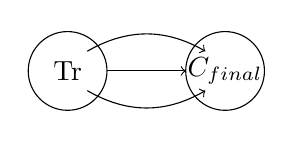
\begin{tikzpicture}
	\draw (-0.5,0) circle(0.5);
	\draw (-0.5,0) node{Tr};
	\draw (1.5,0) circle(0.5);
	\draw (1.5,0) node{$C_{\text{final}}$};
	\draw [->] (0,0)--(1,0);
	\draw [->] (-0.25,-0.25) to[bend right] (1.25,-0.25);
	\draw [->] (-0.25,0.25) to[bend left] (1.25,0.25);
\end{tikzpicture}\end{center}
$\mathcal{L}(X_n)\to \mu_C$, où $\mu_C(j)=0$ $\forall j\in Tr$.\\
$\mu_{C_{|C}}$ = loi de probabilité invariante de la chaîne quand elle début dans C.\\
Sur C, $X_n$ est une chaîne régulière.\\
$\mu=\mu_{C_{|C}}$ vérifie $\mu A=\mu$, $\sum_i \mu_i=1$, dont elle est l'unique solution.
\end{enumerate}

\Theo{ergodique (admis)}{Supposons que la chaîne n'ait qu'une seule classe finale $C$ et que celle-ci est apériodique.\\
Soit $\mu$ la mesure invariante sur $C$ décrite précédemment. Alors :
\[\forall f:E\to \mathbb{R},\ \frac{1}{n} \sum_{k=0}^{n-1} f(X_k) \xrightarrow[\forall \mathcal{L}(X_0)]{p.s.} \int_C f d\mu = \sum_{j\in C} f(j)\mu(j)\]}

\subsection{Etude d'une classe finale périodique}
Soit $d$ la période d'une classe $C$, finale. Elle possède $d$ sous-classes cycliques, parcourues successivement, toujours dans le même ordre. Numérotons les de A à $d$ de façon qu'on les parcourt ainsi :\\
\begin{center}\begin{tikzpicture}
	\draw [->] (0,3)--(1,3);
	\draw (1,5) rectangle (5,1);
	\draw (2,3) node{$C_d$};
	\draw (3,4) node{$C_1$};
	\draw [->] (2.1,3.1) to[bend left] (2.9,3.9);
	\draw (4,3) node{$C_2$};
	\draw [->] (3.1,3.9) to[bend left] (3.9,3.1);
	\draw (3,2) node{$C_k$};
	\draw [->] (3.9,2.9) to[bend left] (3.1,2.1);
	\draw [->] (2.9,2.1) to[bend left] (2.1,2.9);
	\draw (5,1) node[right]{$C$};
\end{tikzpicture}\end{center}

$\Pi$ s'écrit alors :
\[\Pi=\begin{pmatrix} 0 & A_1 & 0 & \cdots & 0 \\
		      0 & 0 & A_2 & \cdots & 0 \\
		      \vdots & \ddots & \ddots & \ddots & \vdots \\
		      0 & 0 & 0 & \cdots & A_{d-1} \\
		      A_d & 0 & 0 & \cdots & 0 \end{pmatrix}\]
\[\Pi^d=\begin{pmatrix} B_1 & 0 & \cdots & 0 \\
			0 & B_2 & \cdots & 0 \\
			\vdots & \vdots & \ddots & \vdots \\
			0 & 0 & \cdots & B_d\end{pmatrix}\]

Avec : \begin{eqnarray*}
	B_1 &=& A_1 \cdots A_d \\
	B_2 &=& A_2 \cdots A_d A_1 \\
	\vdots \\
	B_k &=& A_k \cdots A_d A_1 \cdots A_{k-1} \\
	\vdots \\
	B_d &=& A_d A_1 \cdots A_{d-1}
\end{eqnarray*}

Si on considère $C_k$, $B_k$ est la matrice de transition sur $C_k$. C'est une chaîne de Markov régulière.\\
Elle admet une unique loi de probabilité invariante $\mu_k$ concentrée sur $C_k$. 
	\[\left\{ \begin{array}{c c c} \mu_k B_k &=& \mu_k \\ \sum_{i\in C_k} \mu_k(i) &=& 1 \end{array} \right.\]

\Theo{}{Il existe une unique mesure de probabilité invariante sur C. Notons la $\mu$. On a :
	\[\mu=\frac{1}{d} \left(\mu_1,...,\mu_d \right)\]
$\mu_k$ : vecteur ligne indéxée par $C_k$.}

\begin{dem}
Montrons que $\mu=\frac{1}{d}(\mu_1,...,\mu_d)$ est une mesure de probabilité invariante.
	\[\mu \Pi = \frac{1}{d} (\mu_dA_d , \mu_1A_1, ... , \mu_{d-1}A_{d-1}\]
$\mu_k A_k$ est une mesure de probabilité sur $C_{k+1}$. 
\begin{eqnarray*}
\mu_kA_kB_{k+1}&=&\mu_kA_kA_{k+1}...A_dA_1...A_k \\
		&=& \mu_k B_k A_k\\
		&=& \mu_k A_k
\end{eqnarray*}
Donc $\mu_k A_k=\mu_{k+1}$ par unicité de la loi de probabilité invariante concentrée sur $C_{k+1}$. Donc $\mu\Pi=\mu$.\\
$\mu$ est donc une loi de probabilité invariante.

\bigskip
Prouvons à présent son unicité.\\
Soit $\nu$ une mesure de probabilité invariante.
	\[\nu=(\nu_1,...,\nu_k,...,\nu_d), \nu_k=(\nu_i)_{i\in C_k}\]
	\[\sum_{i\in C_k} \nu_k(i) = \nu(C_k)\]

On a $\nu\Pi=\nu$ donc $\nu\Pi^d=\nu$. donc $\forall k, \nu_kB_k=\nu_k$. Donc :
	\[\frac{\nu_k}{\nu(C_k)} = \mu_k \text{ (par unicité)}\]
Donc $\nu_k=\nu(C_k)\mu_k$.\\

\bigskip
Il reste à montrer que $\forall k$, $\nu(C_k)=\frac{1}{d}$, ie 
	\[\forall k,l, \nu(C_k)=\nu(C_l)\]
car
	\[\sum_{k=1}^d \nu(C_k)=1\]
On a $\nu\Pi=\nu$, donc ::
	\begin{eqnarray*}
		\nu_dA_d&=&\nu_1 \\
		\nu_1A_1&=&\nu_2 \\
		\vdots \\
		\nu_kA_k &=& \nu_{k+1}
	\end{eqnarray*}
\[(\nu_kA_k)_j=\sum_{i\in C_k} \nu_k(i) a_j^i\]
\[\sum_{j\in C_{k+1}} (\nu_k A_k)_j = \sum_{i\in C_k} \nu_k(i) \sum_{j\in C_{k+1}} a^i_j = \sum_{i\in C_k} \nu_k(i) = \nu(C_k)\]
Or, $\nu_kA_k=\nu_{k+1}$ et $\sum_{i\in C_{k+1}} \nu_{k+1}(i)=\nu(C_{k+1})$, donc 
	\[\forall k, \nu(C_k)=\nu(C_{k+1})\]
Ils sont donc tous égaux à $\frac{1}{d}$.
\end{dem}

\Rem{}{\begin{itemize}
	\item Pour cette loi invariante $\mu$, chaque classe $C_k$ a même probabilité $\mu(C_k)=\frac{1}{d}$
	\item Pour trouver $\mu$, 2 méthodes :
	\begin{itemize}
		\item $\mu$ solution de $\mu\Pi=\mu$ et $\sum_{i\in C} \mu_i=1$
		\item On calcule $\Pi^d=diag(B_1,...,B_d)$ et on résout $\mu_kB_k=\mu_k,\ \sum_{i\in C_k} \mu_k(i)=1$. Puis $\mu=\frac{1}{d} (\mu_1,...,\mu_d)$.
	\end{itemize}
	\item Dans la démonstration, au lieu de supposer $\nu$ probabilité invariante, on aurait pu supposer 
		\[\left\{ \begin{array}{c} \nu \text{ solution de } \nu\Pi=\nu \\ \sum \nu_i = 1 \end{array}\right.\]
		Le reste est inchangé.
\end{itemize}}

\Theo{ergodique}{Supposons que la chaîne ne possède qu'une seule classe finale $C$. Soit $\mu_C$ la mesure invariante associée à cette classe. $\forall f:E\to\mathbb{R}$ (E fini) :
\[\frac{1}{n} \sum_{k=1}^n f(X_k) \xrightarrow[\forall \mathcal{L}(X_0)]{p.s.} \int_C f d\mu_C = \sum_{i\in C} f(i)\mu_C(i)\]}
